\documentclass[11pt,a4paper]{article}

\usepackage[utf8]{inputenc}
\usepackage[T1]{fontenc}
\usepackage[spanish]{babel}
\usepackage{booktabs}
\usepackage{listings}
\usepackage{graphicx}
\usepackage[style=ieee,backend=biber,sorting=none]{biblatex}
\usepackage{amsmath}
\usepackage{hyperref}

\usepackage{geometry}
\geometry{margin=2.5cm}
\usepackage{caption}
\usepackage{float}
\usepackage{xcolor}

\addbibresource{referencias.bib}

\hypersetup{
    colorlinks=true,
    linkcolor=blue,
    citecolor=blue,
    urlcolor=blue,
    pdftitle={Analisis de Consistencia y Replicacion en la Base de Datos de TiendaTech},
    pdfauthor={Jeremy Ruperto Gaibor Rodriguez}
}

\lstset{
    basicstyle=\ttfamily\small,
    breaklines=true,
    frame=single,
    backgroundcolor=\color{gray!10},
    numbers=left,
    numberstyle=\tiny,
    keywordstyle=\color{blue},
    commentstyle=\color{gray}
}

\title{\textbf{Análisis de Consistencia y Replicación en la Base de Datos de TiendaTech}}
\author{Jeremy Ruperto Gaibor Rodríguez}
\date{}

\begin{document}

% PORTADA + RESUMEN
\begin{center}
    {\Large \textbf{TA-IND-02}\par}
    \vspace{0.4cm}
    {\Large \textbf{Análisis de Consistencia y Replicación en la Base de Datos de TiendaTech}\par}
    \vspace{0.8cm}

    \begin{tabular}{ll}
        \textbf{Estudiante:} & Jeremy Ruperto Gaibor Rodríguez \\[0.15cm]
        \textbf{Equipo PFC:} & AGLS -- TiendaTech \\[0.15cm]
        \textbf{Asignatura:} & Aplicaciones Distribuidas (ISR-701) \\[0.15cm]
        \textbf{Unidad:} & Unidad 3 -- Bases de Datos Distribuidas \\[0.15cm]
        \textbf{Fecha:} & Julio de 2026 \\
    \end{tabular}
\end{center}

\vspace{1cm}
\hrule
\vspace{0.5cm}

\section*{Resumen}
El presente informe analiza el modelo de consistencia y la estrategia de replicación de TiendaTech, una plataforma de comercio electrónico orientada a la venta de componentes informáticos. La implementación actual emplea una aplicación Spring Boot conectada a una única instancia PostgreSQL 17 desplegada mediante Docker Compose. Por tanto, la persistencia se encuentra centralizada y no existe replicación entre nodos. Esta configuración simplifica las operaciones transaccionales, pero convierte a PostgreSQL en un punto único de fallo. El modelo se evalúa mediante los conceptos de consistencia, CAP y PACELC. También se contrastan tres alternativas: replicación síncrona primario--respaldo, replicación asíncrona con réplicas de lectura y una estrategia híbrida. Se concluye que el diseño actual es adecuado para un prototipo académico, pero no es óptimo para una plataforma productiva que requiera alta disponibilidad. Se recomienda conservar garantías estrictas para inventario, pedidos y pagos, y utilizar réplicas asíncronas para catálogo, búsquedas y reportes.

\vspace{0.3cm}
\noindent\textbf{Palabras clave:} consistencia, replicación, PostgreSQL, CAP, PACELC, TiendaTech.

\newpage
\tableofcontents
\newpage

% INTRODUCCIÓN
\section{Introducción}
TiendaTech es una plataforma de comercio electrónico especializada en componentes informáticos y asistencia para seleccionar productos compatibles. El sistema contempla la gestión de usuarios, catálogo, inventario, carrito de compras, pedidos, ventas y pagos. En este dominio, la persistencia debe evitar resultados contradictorios cuando varias operaciones se ejecutan simultáneamente. Los sistemas distribuidos deben equilibrar consistencia, disponibilidad, latencia y tolerancia a fallos de acuerdo con los requisitos de cada aplicación \cite{margara2023}.

Aunque el diseño del PFC plantea una arquitectura basada en servicios, la persistencia realmente implementada utiliza una única instancia PostgreSQL. El archivo Docker Compose contiene un servicio para la aplicación y otro para la base de datos. No existe un nodo secundario al cual redirigir las operaciones si PostgreSQL deja de responder.

El uso de contenedores o infraestructura en la nube no convierte automáticamente una base de datos en distribuida. Una base distribuida requiere que los datos o las funciones de almacenamiento se encuentren coordinados entre varios nodos \cite{margara2023}.

El objetivo de este informe es caracterizar el modelo de consistencia realmente utilizado en TiendaTech, analizar sus propiedades mediante CAP y PACELC y evaluar alternativas de replicación. La pregunta orientadora es la siguiente:

\begin{quote}
\textit{¿El modelo de consistencia elegido es el óptimo para el dominio de TiendaTech?}
\end{quote}

% MARCO TEÓRICO 
\section{Marco teórico}

\subsection{Modelos de consistencia}
La consistencia determina las restricciones aplicadas al orden y a la visibilidad de las operaciones. No es una propiedad únicamente binaria, sino un espectro de garantías con distintos niveles de fuerza semántica. Viotti y Vukolić organizan estos modelos según las relaciones que establecen entre lecturas, escrituras y procesos \cite{viotti2016}.

La \textbf{linealizabilidad}, también relacionada con la consistencia fuerte, exige que cada operación parezca ejecutarse instantáneamente entre su inicio y su finalización. Una lectura iniciada después de una escritura confirmada debe observar el nuevo valor. Esta garantía facilita el razonamiento sobre la aplicación, pero requiere mayor coordinación cuando existen varias réplicas \cite{viotti2016}.

La \textbf{consistencia secuencial} establece que todos los procesos deben observar las operaciones en un mismo orden global, compatible con el orden de cada proceso. A diferencia de la linealizabilidad, ese orden no tiene que corresponder exactamente con el tiempo real \cite{viotti2016}.

La \textbf{consistencia causal} conserva el orden entre operaciones relacionadas por causa y efecto. Cuando una operación depende de otra, todos los nodos deben observarlas en ese mismo orden. Las operaciones concurrentes sin relación causal pueden ser observadas de manera diferente \cite{viotti2016}.

La garantía de lectura de los propios cambios, conocida como \textbf{read-your-writes}, asegura que un usuario pueda observar sus propias modificaciones posteriores. Esta propiedad evita que, después de actualizar un perfil o agregar un producto al carrito, la misma sesión reciba una versión anterior \cite{viotti2016}.

La \textbf{consistencia eventual} permite que las réplicas presenten diferencias temporales. Si dejan de producirse escrituras, todas las copias terminan convergiendo. Esta garantía puede mejorar la disponibilidad y reducir la coordinación, pero admite lecturas temporalmente desactualizadas \cite{viotti2016}.

En términos generales, los modelos más fuertes requieren mayor coordinación, mientras que los modelos más débiles permiten reducir la latencia y favorecer la disponibilidad. Las propuestas recientes buscan disminuir el costo de coordinación sin renunciar por completo a garantías fuertes \cite{margara2023,zhou2023}.

\subsection{Teorema CAP}
CAP relaciona tres propiedades: consistencia, disponibilidad y tolerancia a particiones. Gilbert y Lynch demostraron que, cuando una partición impide la comunicación entre nodos, no es posible garantizar simultáneamente consistencia y disponibilidad \cite{gilbert2002}.

Esto no significa que un sistema seleccione permanentemente dos características de tres. La decisión se presenta específicamente durante una partición. El sistema puede rechazar operaciones para impedir divergencias o continuar respondiendo y aceptar estados temporalmente diferentes \cite{gilbert2002}.

En TiendaTech no existe actualmente una partición entre réplicas porque solo hay una instancia PostgreSQL. Si la aplicación pierde el acceso a ese nodo, no dispone de otra copia operativa y deja de estar disponible.

\subsection{PACELC}
PACELC amplía CAP al considerar que los compromisos también están presentes durante la operación normal. Si existe una partición, debe elegirse entre disponibilidad y consistencia; si no existe una partición, se presenta un compromiso entre latencia y consistencia \cite{abadi2012}.

En una \textbf{replicación síncrona}, la transacción espera que otro nodo reciba o confirme la modificación antes de finalizar. Esta espera reduce el riesgo de que una operación confirmada exista únicamente en el nodo principal, pero añade comunicación y aumenta el tiempo de respuesta \cite{abadi2012,margara2023}.

En una \textbf{replicación asíncrona}, el nodo principal puede confirmar primero y actualizar después a los seguidores. Esto reduce la latencia de escritura, pero permite que una réplica muestre temporalmente un valor anterior \cite{abadi2012,margara2023}.

En TiendaTech, inventario, pedidos y pagos justifican una mayor coordinación porque una inconsistencia podría causar sobreventa, pedidos incompletos o cobros duplicados. Las imágenes, descripciones, recomendaciones y reportes pueden tolerar retrasos breves. Esta distinción corresponde a un análisis propio de los requisitos del dominio.

\subsection{Estrategias de replicación}
La replicación consiste en mantener copias de los datos en varios nodos para mejorar disponibilidad, tolerancia a fallos y capacidad de lectura. Sin embargo, cada copia adicional introduce la necesidad de propagar, ordenar y confirmar modificaciones \cite{margara2023}.

En la replicación \textbf{primario--seguidor}, un nodo principal recibe las escrituras y transmite los cambios a uno o varios nodos secundarios. Los seguidores pueden atender consultas y uno de ellos podría sustituir al primario si la arquitectura incorpora mecanismos adicionales de detección de fallos, promoción y redirección de conexiones \cite{margara2023}.

La replicación \textbf{multi-líder} permite que varios nodos acepten escrituras. Puede reducir la latencia para usuarios ubicados en regiones diferentes, pero genera el riesgo de modificaciones concurrentes sobre los mismos datos. GeoGauss utiliza una arquitectura multi-maestro que combina replicación y control de concurrencia para conservar consistencia fuerte con menor coordinación \cite{zhou2023}.

En la replicación \textbf{sin líder}, las operaciones se distribuyen entre diferentes copias mediante quórums de lectura y escritura, sin depender permanentemente de un nodo principal. Esta estrategia favorece la disponibilidad, pero obliga a manejar versiones concurrentes y reconciliación de datos \cite{decandia2007}.

Dynamo constituye un caso representativo de replicación sin líder. Su diseño distribuye los datos entre varios nodos, emplea cantidades configurables de réplicas para lectura y escritura y permite reconciliar posteriormente versiones concurrentes. El sistema prioriza disponibilidad y tolerancia a fallos, aceptando consistencia eventual \cite{decandia2007}.

La replicación también puede ser síncrona o asíncrona. En la modalidad síncrona, la confirmación espera la participación de otro nodo. En la modalidad asíncrona, el primario responde antes de que todas las copias se actualicen. La primera ofrece mayor protección de las operaciones confirmadas; la segunda reduce la latencia, pero admite retraso entre réplicas \cite{abadi2012,margara2023}.

\subsection{Estado del arte}
Margara et al. presentan un modelo para estudiar sistemas distribuidos intensivos en datos según aspectos como distribución, procesamiento, consistencia, recuperación y coordinación. Su revisión muestra que no existe una arquitectura universalmente superior, porque cada sistema combina garantías y costos según sus objetivos \cite{margara2023}.

GeoGauss propone una base de datos SQL geo-replicada con arquitectura multi-maestro y consistencia fuerte. Su diseño combina replicación, procesamiento por épocas y control optimista de concurrencia con el propósito de reducir la coordinación entre regiones \cite{zhou2023}.

PolyBase analiza la influencia de la ubicación geográfica de los líderes y de los grupos de consenso sobre la latencia. La propuesta permite reasignar filas entre grupos de replicación para acercarlas a las regiones desde las cuales reciben más solicitudes \cite{ruan2024}.

Stabilizer permite que la aplicación defina las garantías de consistencia requeridas para determinadas operaciones. Este planteamiento resulta pertinente para TiendaTech porque los datos de inventario y pagos no requieren las mismas garantías que las recomendaciones o los reportes \cite{li2022}.

Dynamo y Spanner representan dos extremos del espectro. Dynamo prioriza disponibilidad mediante replicación sin líder y consistencia eventual \cite{decandia2007}. Spanner ofrece consistencia externa para transacciones distribuidas mediante replicación coordinada y sincronización temporal \cite{corbett2013}.

La comparación entre ambos sistemas demuestra que no existe una estrategia única para todos los dominios. Dynamo acepta divergencias temporales para continuar respondiendo, mientras que Spanner asume un mayor costo de coordinación para proporcionar un orden global más estricto \cite{corbett2013,decandia2007}.

Para TiendaTech, una arquitectura completamente eventual sería riesgosa para inventario, pedidos y pagos. En el extremo contrario, una infraestructura global comparable con Spanner sería excesiva para el alcance actual del proyecto. La solución debe aplicar garantías diferentes según la criticidad de los datos. Esta conclusión constituye un análisis propio del dominio apoyado en los compromisos descritos por las fuentes anteriores.

% ANÁLISIS DEL MODELO
\section{Análisis del modelo implementado en TiendaTech}

\subsection{Caracterización de la implementación}
La implementación utiliza una única instancia PostgreSQL 17. El Docker Compose define el contenedor \texttt{tiendatech\_postgres}, expuesto en el puerto 5432, y el contenedor \texttt{tiendatech\_app}, expuesto en el puerto 8080.

La aplicación depende directamente del servicio PostgreSQL. No existen configuraciones de nodos secundarios, quórum, consenso, replicación ni promoción automática.

El volumen \texttt{postgres\_data} conserva los archivos de PostgreSQL cuando el contenedor se reinicia o se vuelve a crear. Sin embargo, no constituye una réplica porque no mantiene una segunda instancia operativa.

La caracterización correcta del modelo es:

\begin{quote}
\textit{TiendaTech utiliza una base de datos PostgreSQL centralizada, con consistencia transaccional local y sin una estrategia de replicación implementada.}
\end{quote}

\subsection{Topología de persistencia}
La Figura~\ref{fig:topologia} presenta la topología realmente implementada. El usuario accede a la aplicación, esta realiza operaciones mediante JDBC/SQL y PostgreSQL conserva sus archivos en el volumen Docker.

\begin{figure}[H]
    \centering
    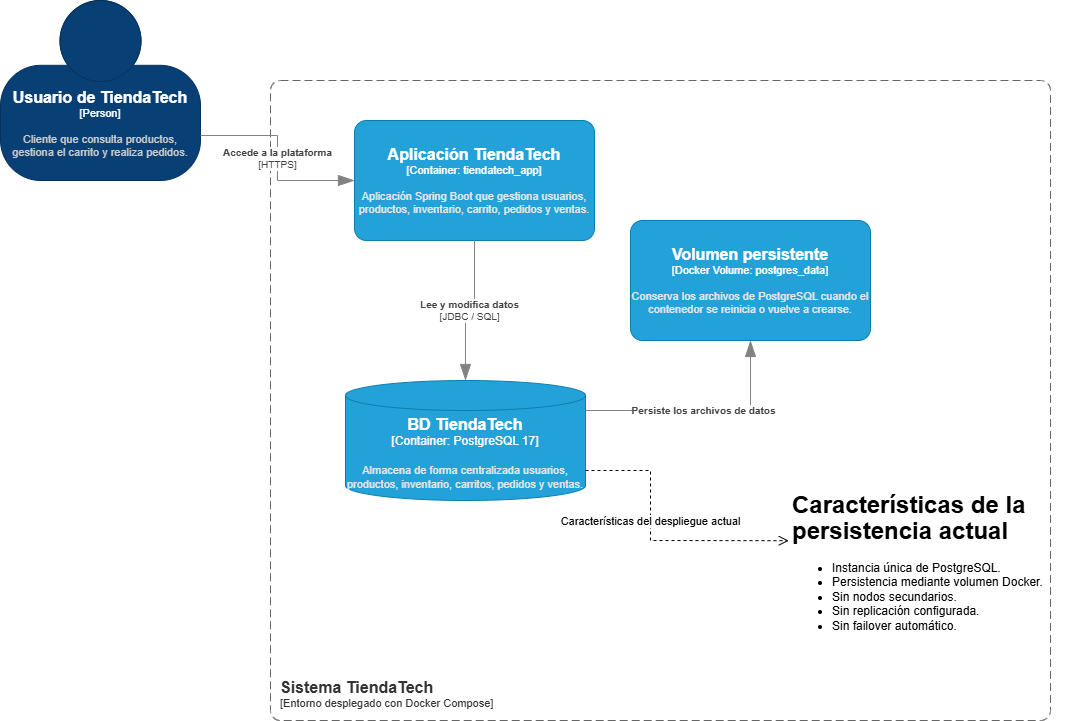
\includegraphics[width=0.95\textwidth]{imagenes/topologia_actual_tiendatech.png}
    \caption{Topología actual de persistencia de TiendaTech. Fuente: elaboración propia.}
    \label{fig:topologia}
\end{figure}

Como se observa en la Figura~\ref{fig:topologia}, PostgreSQL constituye el único nodo de datos. No existen nodos secundarios, replicación ni \textit{failover} automático.

El volumen persistente protege la información frente a la recreación del contenedor, pero continúa dependiendo del mismo servidor. Si se pierde la máquina, el almacenamiento o la instancia PostgreSQL, la aplicación no puede utilizar otra copia.

\subsection{Modelo de consistencia identificado}
TiendaTech obtiene consistencia transaccional local porque todas las operaciones se ejecutan sobre una misma instancia PostgreSQL. No existe retraso de propagación entre réplicas.

No sería correcto afirmar que el sistema implementa linealizabilidad distribuida, debido a que no existen varios nodos coordinados. Tampoco puede asegurarse que todas las transacciones sean serializables sin revisar el nivel de aislamiento configurado.

La ventaja del nodo único es que no aparecen conflictos entre copias. La limitación es que la consistencia se obtiene sin redundancia y toda la aplicación depende de la disponibilidad de PostgreSQL.

\subsection{Estrategia de replicación actual}
La estrategia de replicación implementada es \textbf{inexistente}. Esta conclusión se basa en el Docker Compose, donde solamente se declara un contenedor PostgreSQL:

\begin{lstlisting}[caption={Fragmento representativo del Docker Compose de TiendaTech}, label={lst:compose}]
services:
  tiendatech_app:
    build: .
    ports:
      - "8080:8080"
    depends_on:
      - tiendatech_postgres
    restart: always

  tiendatech_postgres:
    image: postgres:17
    ports:
      - "5432:5432"
    volumes:
      - postgres_data:/var/lib/postgresql/data
    restart: always

volumes:
  postgres_data:
\end{lstlisting}

La ausencia de replicación reduce la complejidad, el consumo de recursos y el esfuerzo de administración. Esta decisión resulta comprensible durante una etapa académica inicial.

Sin embargo, PostgreSQL se convierte en un punto único de fallo. La opción \texttt{restart: always} intenta reiniciar el mismo contenedor, pero no reemplaza el nodo si falla el servidor o el almacenamiento.

\subsection{Requisitos de consistencia del dominio}
El inventario requiere garantías estrictas. Si dos usuarios intentan comprar la última unidad y la comprobación del \textit{stock} no se coordina correctamente, el sistema podría aceptar una sobreventa. Por ello, la lectura, comprobación y disminución del \textit{stock} deben formar parte de una operación transaccional coherente.

Los sistemas OLTP geo-replicados muestran que la modificación concurrente de datos compartidos requiere mecanismos de coordinación y control de concurrencia \cite{zhou2023}.

Los pedidos y las ventas necesitan atomicidad para evitar registros parciales. La cabecera, los detalles, el total y la actualización de existencias deben mantenerse coherentes. Esta necesidad se deriva directamente de las reglas de negocio de TiendaTech.

Los pagos requieren idempotencia y almacenamiento consistente para impedir cobros duplicados. Los usuarios, roles y credenciales también necesitan que las modificaciones relevantes sean visibles rápidamente.

El catálogo, las imágenes y los reportes pueden tolerar retrasos breves. Mostrar temporalmente una descripción anterior tiene menor impacto que confirmar una compra sin \textit{stock}.

La literatura reciente sobre consistencia definida por la aplicación respalda la posibilidad de emplear garantías diferentes según el tipo de operación \cite{li2022}.

\begin{table}[H]
    \centering
    \caption{Nivel de consistencia requerido por tipo de dato en TiendaTech}
    \label{tab:requisitos}
    \begin{tabular}{@{}ll@{}}
        \toprule
        \textbf{Nivel requerido} & \textbf{Datos principales} \\
        \midrule
        Consistencia estricta   & Inventario, pedidos, pagos, ventas, credenciales y roles \\
        Tolerancia limitada     & Productos, categorías, marcas, imágenes y búsquedas \\
        Consistencia eventual   & Estadísticas, recomendaciones y reportes analíticos \\
        \bottomrule
    \end{tabular}
\end{table}

\subsection{Análisis mediante CAP}
En la topología actual no existe una partición entre réplicas porque solamente se utiliza una instancia PostgreSQL. Si la aplicación pierde acceso al nodo, el servicio de datos deja de estar disponible.

El diseño evita divergencias entre copias, pero no ofrece tolerancia frente al fallo del nodo. Si se incorporaran réplicas, inventario y pagos deberían priorizar consistencia durante una partición, mientras que catálogo y reportes podrían mantener disponibilidad mediante lecturas temporalmente atrasadas. Esta decisión se relaciona con el compromiso formal planteado por CAP \cite{gilbert2002}.

\subsection{Análisis mediante PACELC}
Durante el funcionamiento normal, TiendaTech no espera confirmaciones remotas, lo que reduce la latencia.

Una réplica síncrona aumentaría el tiempo de confirmación porque la escritura debería esperar la participación de otro nodo. Una réplica asíncrona reduciría ese tiempo, pero podría entregar valores anteriores. Este compromiso corresponde al equilibrio entre latencia y consistencia descrito por PACELC \cite{abadi2012}.

La ubicación de los líderes y de los grupos de consenso también puede influir en el costo de comunicación y en la latencia de las operaciones \cite{ruan2024}.

La decisión más adecuada consiste en aplicar garantías fuertes a los procesos críticos y permitir menor coordinación en consultas que toleren retrasos. Esta postura se fundamenta en los requisitos específicos de TiendaTech.

% EVALUACIÓN DE ALTERNATIVAS
\section{Evaluación de alternativas}

\subsection{Primario con respaldo síncrono}
Esta alternativa mantiene un PostgreSQL primario y agrega un nodo de respaldo. Las transacciones críticas se confirman después de que el secundario recibe la modificación.

La replicación síncrona reduce el riesgo de que una operación confirmada exista únicamente en el nodo principal, aunque añade comunicación y tiempo de espera \cite{abadi2012,margara2023}.

Esta estrategia resulta apropiada para inventario, pedidos y pagos. Su desventaja es el incremento de latencia y la necesidad de implementar detección de fallos, promoción del secundario y redirección de conexiones.

\subsection{Primario con réplica asíncrona}
Esta alternativa conserva un primario para las escrituras y añade uno o varios seguidores para las lecturas.

Las réplicas podrían atender consultas de catálogo, imágenes, búsquedas y reportes. Sin embargo, pueden mostrar información temporalmente atrasada, por lo que no deberían utilizarse para confirmar el \textit{stock} definitivo de una compra.

La ventaja principal es que se distribuye la carga de lectura sin obligar al primario a esperar la confirmación de todos los seguidores \cite{margara2023}.

\subsection{Estrategia híbrida}
La estrategia híbrida combinaría:

\begin{itemize}
    \item un nodo primario para todas las escrituras;
    \item un respaldo síncrono para operaciones críticas;
    \item una réplica asíncrona para catálogo y reportes;
    \item un mecanismo de \textit{failover};
    \item monitoreo del retraso de replicación;
    \item copias de seguridad externas.
\end{itemize}

Esta alternativa diferencia las garantías según la criticidad de los datos, principio relacionado con la consistencia definida por la aplicación \cite{li2022}.

Ofrece un mejor equilibrio entre consistencia, disponibilidad y rendimiento, aunque incrementa la complejidad de administración y enrutamiento de consultas.

\subsection{Tabla comparativa}

\begin{table}[H]
    \centering
    \caption{Comparación entre el modelo actual y las alternativas evaluadas}
    \label{tab:comparativa}
    \resizebox{\textwidth}{!}{%
    \small
    \begin{tabular}{@{}lllll@{}}
        \toprule
        \textbf{Criterio} & \textbf{Nodo único} & \textbf{Respaldo síncrono} & \textbf{Réplica asíncrona} & \textbf{Estrategia híbrida} \\
        \midrule
        Consistencia              & Local             & Alta               & Alta en el primario & Alta en datos críticos \\
        Disponibilidad            & Baja              & Alta con failover  & Alta para lecturas  & Alta \\
        Latencia de escritura     & Baja              & Mayor              & Baja                & Media \\
        Latencia de lectura       & Limitada          & Media              & Baja                & Ajustada al dato \\
        Tolerancia a fallos       & Baja              & Alta               & Media               & Alta \\
        Tolerancia a particiones & No implementada   & Prioriza consistencia & Mantiene lecturas & Depende del proceso \\
        Riesgo de datos atrasados & No aplica         & Muy bajo           & Presente            & Controlado \\
        Escalabilidad de lectura  & Limitada          & Media              & Alta                & Alta \\
        Complejidad operativa     & Baja              & Media              & Media               & Alta \\
        Adecuación general        & Prototipo         & Datos críticos     & Consultas no críticas & Producción \\
        \bottomrule
    \end{tabular}%
    }
\end{table}

% DISCUSIÓN CRÍTICA
\section{Discusión crítica}

\subsection{¿Es óptimo el modelo actual?}
El modelo actual es adecuado para una etapa académica porque simplifica el desarrollo y evita problemas de sincronización entre réplicas.

Sin embargo, no es óptimo para una plataforma productiva. PostgreSQL constituye un punto único de fallo y todas las operaciones dependen de su disponibilidad.

El volumen Docker conserva los archivos de la base, pero no proporciona una segunda instancia operativa. De igual manera, \texttt{restart: always} intenta reiniciar el mismo contenedor y no ejecuta \textit{failover} hacia otro servidor.

Por tanto:

\begin{quote}
\textit{El modelo centralizado es suficiente para el prototipo actual, pero no es óptimo para una versión productiva que requiera alta disponibilidad, escalabilidad y tolerancia a fallos.}
\end{quote}

\subsection{Trade-offs}
El primer compromiso es simplicidad frente a disponibilidad. Una instancia única es sencilla de administrar, pero su falla detiene toda la persistencia.

El segundo compromiso es latencia frente a durabilidad. Una confirmación síncrona protege mejor las transacciones, pero añade comunicación y tiempo de espera \cite{abadi2012}.

El tercero es disponibilidad frente a actualidad de las lecturas. Una réplica asíncrona puede distribuir consultas, pero podría entregar valores temporalmente anteriores \cite{margara2023}.

El cuarto es consistencia uniforme frente a consistencia diferenciada. Aplicar coordinación fuerte a todos los datos sería innecesario, mientras que aplicar consistencia eventual al inventario y a los pagos sería riesgoso. La consistencia definida según la aplicación permite adaptar las garantías a cada tipo de dato \cite{li2022}.

\subsection{Limitaciones}
Las principales limitaciones identificadas son:

\begin{itemize}
    \item Punto único de fallo.
    \item Ausencia de \textit{failover} automático.
    \item Escalabilidad horizontal limitada.
    \item Dependencia del mismo servidor y volumen.
    \item Posibles interrupciones durante mantenimiento.
    \item Falta de redundancia operativa.
    \item Imposibilidad de distribuir las lecturas.
\end{itemize}

\subsection{Mitigaciones}
Se proponen las siguientes medidas:

\begin{enumerate}
    \item Mantener transacciones para controlar la comprobación y reducción del \textit{stock}.
    \item Incorporar inicialmente una réplica asíncrona.
    \item Evaluar un respaldo síncrono para pagos y pedidos.
    \item Mantener copias de seguridad externas.
    \item Monitorear la disponibilidad y el retraso de replicación.
    \item Implementar idempotencia en pagos y creación de pedidos.
    \item Probar periódicamente los procedimientos de \textit{failover} y restauración.
\end{enumerate}

\subsection{Propuesta recomendada}
La propuesta recomendada es una evolución híbrida y progresiva. Primero se añadiría una réplica asíncrona para catálogo, reportes y recuperación. Posteriormente, se incorporaría un respaldo síncrono para proteger inventario, pedidos y pagos.

Las consultas críticas permanecerían en el primario, mientras que las consultas tolerantes a retrasos podrían dirigirse a las réplicas.

Esta alternativa reduce progresivamente el punto único de fallo sin introducir desde el inicio la complejidad de una arquitectura multi-líder.

% CONCLUSIONES
\section{Conclusiones}
TiendaTech utiliza una única instancia PostgreSQL y no posee replicación. Su modelo corresponde a una persistencia centralizada con consistencia transaccional local.

La solución es adecuada para un prototipo académico, pero presenta un punto único de fallo y no garantiza continuidad operativa.

El análisis mediante CAP muestra que, al perder el acceso a PostgreSQL, la aplicación deja de estar disponible. PACELC permite observar que la baja latencia actual se obtiene al no coordinar varias réplicas.

La replicación síncrona resulta apropiada para inventario, pedidos y pagos, aunque incrementa la latencia. La replicación asíncrona puede mejorar la capacidad de lectura del catálogo y de los reportes, pero admite información temporalmente atrasada.

El modelo actual no es óptimo para una versión productiva. La alternativa recomendada es una estrategia híbrida que combine garantías fuertes para los procesos críticos y réplicas asíncronas para las lecturas no críticas.

% DECLARACIÓN DE USO DE IA
\section{Declaración de uso de inteligencia artificial generativa}
Para la elaboración de este informe se utilizó ChatGPT como herramienta de apoyo en la organización de la estructura del documento, la revisión de la claridad de la redacción y la presentación de algunas ideas técnicas. La asistencia se aplicó principalmente en las secciones de marco teórico, evaluación de alternativas, discusión crítica y conclusiones.

El análisis de la arquitectura de TiendaTech, la comprobación de la implementación, la interpretación de las fuentes, la selección de la propuesta y la revisión final fueron realizadas por el autor.

% REFERENCIAS 
\printbibliography[title={Referencias}]

\end{document}